%%%%%%%%%%%%%%%%%%%%%%%%%%%%%%%%%%%%%%%%
% iz predloge:
%
% datoteka diploma-vzorec.tex
%
% vzorčna datoteka za pisanje diplomskega dela v formatu LaTeX
% na UL Fakulteti za računalništvo in informatiko
%
% vkup spravil Gašper Fijavž, december 2010
% množica popravkov v januarju, februarju marcu 2011
% verzija 29. marec 2011

\documentclass[a4paper, 12pt, ]{book} 
%openany?

\usepackage[utf8x]{inputenc}   % omogoča uporabo slovenskih črk kodiranih v formatu UTF-8 
\usepackage[slovene,english]{babel}    % naloži, med drugim, slovenske delilne vzorce
\usepackage[pdftex]{graphicx}  % omogoča vlaganje slik različnih formatov 
\usepackage{fancyhdr}          % poskrbi, na primer, za glave strani
\usepackage{amssymb}           % dodatni simboli
\usepackage{amsmath}           % eqref, npr.

\usepackage{color}		% barve

\usepackage{hyphenat}
\usepackage{hyperref}	% povezave
\hypersetup{
    colorlinks=false, 		%set true if you want colored links
    linktoc=all,    			 %set to all if you want both sections and subsections linked
    colorlinks,
    citecolor=black,
    filecolor=black,
    linkcolor=black,
    urlcolor=black
}
\usepackage[hmarginratio=3:2]{geometry}	% obrne razmerja marginov
\usepackage[nottoc]{tocbibind}	% prepreči številko za literaturo v kazalu
\usepackage{amssymb}		% oznake za množice števil, npr. N za naravna števila

%---------------------------------------------
% pseudokoda
\usepackage[chapter]{algorithm}
\usepackage[noend]{algpseudocode}
%\usepackage{algorithmicx}
\usepackage{setspace}
\newcommand{\alglinestretch}{1}
\floatname{algorithm}{Algoritem}
\renewcommand{\algorithmicrequire}{\textbf{Vhod:}}
\renewcommand{\algorithmicensure}{\textbf{Izhod:}}
%---------------------------------------------




\renewcommand{\baselinestretch}{1.3} % ustrezen razmik med vrsticami

%oznake strani
\renewcommand{\chaptermark}[1]{\markboth{\MakeUppercase{\thechapter.\ #1}}{}}
\renewcommand{\sectionmark}[1]{\markright{\MakeUppercase{\thesection.\ #1}}}
\renewcommand{\headrulewidth}{0.5pt}
\renewcommand{\footrulewidth}{0pt} 
\fancyhf{}
\fancyhead[LE,RO]{\sl \thepage}
\fancyhead[LO]{\sl \rightmark}
\fancyhead[RE]{\sl \leftmark}


\newcommand{\BibTeX}{{\sc Bib}\TeX}

\newcommand{\autfont}{\Large}
\newcommand{\titfont}{\LARGE\bf}

\setcounter{tocdepth}{1}	      % globina kazala

% konstrukti
\newtheorem{izrek}{Izrek}[chapter]
%\newtheorem{trditev}{Trditev}[izrek]
\newenvironment{dokaz}{\emph{Dokaz.}\ }{\hspace{\fill}{$\Box$}}

% todo tag
\newcommand{\TODO}[1]{\textcolor{red}{#1}}

\newcommand{\clearemptydoublepage}{\newpage{\pagestyle{empty}\cleardoublepage}}







\begin{document}
\selectlanguage{slovene}
\frontmatter
\setcounter{page}{1} %
\renewcommand{\thepage}{}       % preprecimo težave s številkami strani v kazalu 



	%---------------------------------------------
	%naslovnica
	 \thispagestyle{empty}%
	   \begin{center}
	    {\large\sc Univerza v Ljubljani\\%
	      Fakulteta za računalništvo in informatiko}%
	    \vskip 10em%
	    {\autfont Nejc Ramovš\par}%
	    {\titfont Problem izomorfnega podgrafa \par}%
	    {\vskip 2em \textsc{DIPLOMSKO DELO\\NA UNIVERZITETNEM ŠTUDIJU}\par}%
	    \vfill\null%
	    {\large \textsc{Mentor}: prof.~dr.~Borut Robič\par}%
	    {\vskip 2em \large Ljubljana, 2013 \par}%
	\end{center}
	
	% prazna stran
	\clearemptydoublepage




	%---------------------------------------------
	%copyright stran
	\thispagestyle{empty}
	\vspace*{8cm}
	{\small \noindent
	Rezultati diplomskega dela so intelektualna lastnina Fakultete za ra\-ču\-nal\-niš\-tvo in informatiko Univerze v Ljubljani. 
	Za objavljanje ali izkoriščanje rezultatov di\-plom\-ske\-ga dela je potrebno pisno soglasje Fakultete za ra\-ču\-nal\-niš\-tvo in 
	informatiko ter mentorja.}
	
	% prazna stran
	\clearemptydoublepage
	



	%---------------------------------------------
	% stran 3 med uvodnimi listi
	\noindent
	Namesto te strani {\bf vstavite} original izdane teme diplomskega 
	dela s podpisom mentorja in dekana ter žigom fakultete, ki ga diplomant
	dvigne v študent\-skem referatu,  preden odda izdelek v vezavo!
	
	% prazna stran
	\clearemptydoublepage




	%---------------------------------------------
	% izjava o avtorstvu
	\vspace*{1cm}
	\begin{center} 
	{\Large \textbf{\sc Izjava o avtorstvu diplomskega dela}}
	\end{center}
	
	\vspace{1cm}
	
	\begin{tabbing}
	\hspace*{4cm}\= \kill
	Spodaj podpisani \> Nejc Ramovš,  \\[0.3cm]
	z vpisno številko \>  63070162, \\
	\end{tabbing}
	
	\noindent sem avtor  diplomskega dela z naslovom:
	 
	
	\vspace{0.5cm}
	\emph{Problem izomorfnega podgrafa}
	
	\vspace{1.5cm}
	\noindent S svojim podpisom zagotavljam, da:
	\begin{itemize}
		\item sem diplomsko delo izdelal samostojno pod mentorstvom\\ prof.~dr.~Boruta Robiča,
	
		\item	so elektronska oblika diplomskega dela, naslov (slov., angl.), povzetek (slov., angl.) ter 
		ključne besede (slov., angl.) identični s tiskano obliko diplomskega dela

		\item soglašam z javno objavo elektronske oblike diplomskega dela v zbirki ''Dela FRI''.
	\end{itemize}
	
	\vspace{1cm}
	\noindent V Ljubljani, dne \TODO{09.01.2012} \hspace{3cm} Podpis avtorja:
	
	% prazna stran
	\clearemptydoublepage
	
	
	
	
	%---------------------------------------------
	% zahvala
	\thispagestyle{empty}\mbox{}\vfill\null\it%
	\TODO {Na tem mestu zapišite, komu se zahvaljujete za izdelavo diplomske naloge. Pazite, da ne
	boste koga pozabili. Utegnil vam bo zameriti. Temu se da izogniti tako, da pozabite na celo zahvalo.}
	\rm\normalfont
	
	% prazna stran
	\clearemptydoublepage
	
	
	%---------------------------------------------
	% kazalo
	\def\thepage{}% preprecimo tezave s stevilkami strani v kazalu 
	\tableofcontents{}
	
	% prazna stran
	\clearemptydoublepage
	

	
	
	
	%---------------------------------------------
	% povzetek 
	\chapter*{Povzetek}
	\TODO{V vzorcu je predstavljen postopek priprave diplomskega dela z uporabo okolja \LaTeX.
	Vaš povzetek mora sicer vsebovati približno 100 besed, ta tukaj je odločno prekratek.}
	
	\vspace{2cm}
	\noindent{\large \textbf{Ključne besede:}}\\
	graf
	
	
	% prazna stran
	\clearemptydoublepage
	
	
	
	
	
	%---------------------------------------------
	% abstract
	\selectlanguage{english}
	\chapter*{Abstract}
	\TODO{This sample document presents an approach to typesetting your BSc thesis using \LaTeX. A 
	proper abstract should contain around 100 words which makes this one way too short.}
	\selectlanguage{slovene}
	
	\vspace{2cm}
	\noindent{\large \textbf{Key words:}}\\
	graph
	
	% prazna stran
	\clearemptydoublepage




%%%%%%%%%%%%%%%%%%%%%%%%%%%%%%%%%%%%%%%%
\mainmatter
\setcounter{page}{1}
\pagestyle{fancy}



\chapter{Uvod}





\chapter{Definicija problema}

	\section{Graf}
	Graf $G = \langle V, E \rangle$ je definiran z množico vozlišč $V$ (ang.~vertices) in množico povezav $E$ (ang.~edges). Povezava je par vozlišč: 
	$E \subseteq V \times V$. Kardinalnost $V$ označimo z $n$, kardinalnost $E$ pa z $m$.
	Vozlišči, ki sta vsebovani v povezavi, sta sosednji (ang.~adjacent). Graf je lahko usmerjen (ang.~directed) ali neusmerjen
	(ang.~undirected). V neusmerjenem
	grafu je ena povezava neurejen par vozlišč $u, v \in V$ in jo označimo z $\{u, v\}$. V usmerjenem grafu je povezava urejen par 
	vozlišč $u, v \in V$, kjer je prvo vozlišče začetek (ang.~head), drugo pa konec (ang.~tail) povezave. Označimo jo z $(u, v)$.
	Graf z oznakami $G = (V, E, \alpha, \beta)$ sestavlja graf $(V, E)$, funkcija $\alpha: V \to \mathbb{N} $, ki pripisuje oznako
	vozliščem in funkcija $\beta: E \rightarrow \mathbb{N}$, ki pripisuje oznako povezavam.



	\section{Podgrafni izomorfizem}
	Graf $G' = \langle V', E' \rangle$ je podgraf danega grafa $G = \langle V, E \rangle$, če velja $V' \subseteq V \wedge E' \subseteq E$. 
	Graf $G' = \langle V', E' \rangle$ je induciran podgraf danega grafa $G = \langle V, E \rangle$, če vsebuje vse povezave, katerih vozlišča so
	v $V'$, oz. če velja $E' = E \cap (V' \times V')$.

	Grafa $G_p = \langle V_p, E_p \rangle $ in $G_t = \langle V_t, E_t \rangle$ sta izomorfna, če obstaja bijektivna preslikava $f: V_p \to V_t$ da velja: 
	$(a,b) \in E_p \Leftrightarrow (f(a), f(b)) \in E_t;$
	oznaka $p$ pomeni vzorčni (ang.~pattern) graf, oznaka $t$ pa ciljni (ang.~target) graf. V primeru grafa z oznakami, mora preslikovalna funkcija
	ohranjati oznake. Primer izomorfizma grafov je podan na sliki~\ref{pic_iso}.

	\begin{figure}
	\begin{center}
	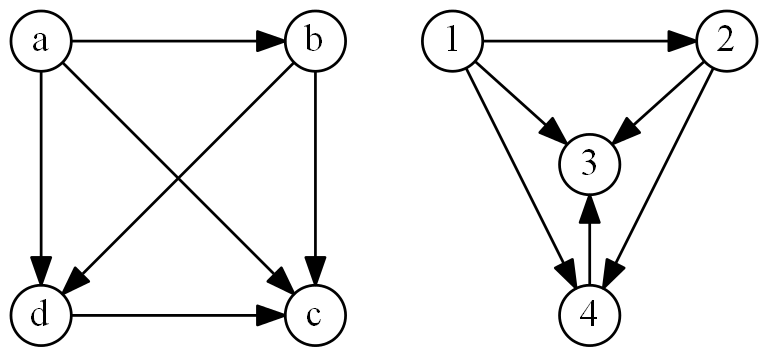
\includegraphics[width=10cm]{img/graph_izomorph.png}
	\end{center}
	\caption{Primer izomorfnih grafov z bijektivno funkcijo $f = \{(a, 1), (b, 2), (c, 3), (d, 4)\}$.}
	\label{pic_iso}
	\end{figure}


	Graf $G_p$ je izomorfen podgraf grafa $G_t$, če obstaja podgraf $G_t'$ grafa $G_t$, ki je izomorfen grafu $G_p$.
	Med grafoma $G_p$ in $G_t$ obstaja parcialen podgrafni izomorfizem, če je funkcija $f: V_p \to V_t$ injektivna in velja
	$(a,b) \in E_p \Rightarrow (f(a), f(b)) \in E_t$.
	Med grafoma $G_p$ in $G_t$ obstaja induciran podgrafni izomorfizem, če je funkcija $f: V_p \to V_t$ injektivna in velja
	$(a,b) \in E_p \Leftrightarrow (f(a), f(b)) \in E_t$. Na sliki~\ref{pic_sub_iso} vidimo, da je med $b)$ in $c)$ samo parcialni podgrafni
	izomorfizem, ker v vzorčnem grafu ni povezave $(B, C)$, medtem ko preslikavi teh vozlišč $(2, 3)$ tvorita povezavo v $c)$. Induciran 
	podgrafni izomorfizem lahko obstaja samo, če se ohranijo tudi ne-povezave.
	
	Pri reševanju problema izomorfnega podgrafa lahko ugotavljamo obstoj oz.~število podgrafnih izomorfizmov ali pa iščemo enega oz.~vse
	podgrafne izomorfizme (preslikave $f$). Najtežja je generiranje vseh preslikav - to različico rešujejo opisani algoritmi. Dodatno lahko rešujemo
	problem še na usmerjenih ali neusmerjenih ter označenih ali neoznačenih grafih.


	\begin{figure}
	\begin{center}
	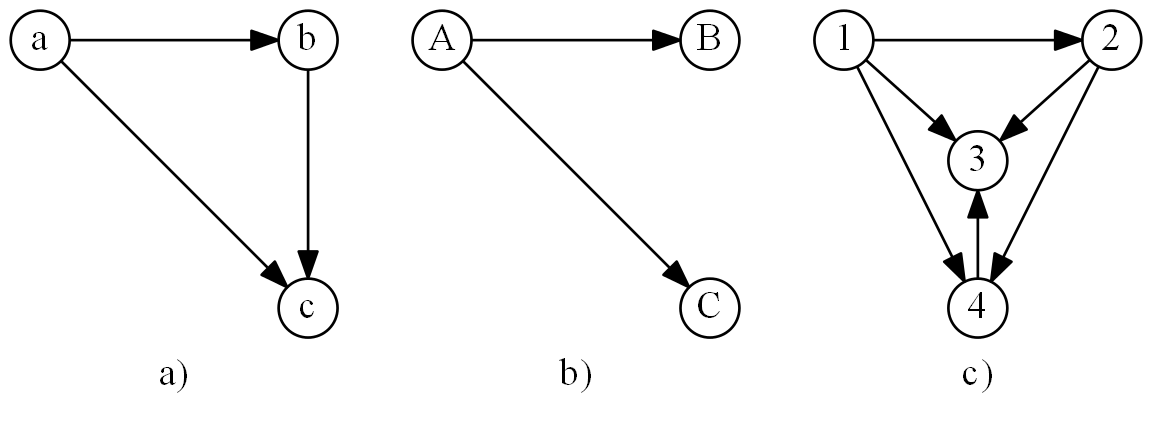
\includegraphics[width=15cm]{img/graph_sub_izomorph.png}
	\end{center}
	\caption{Med $a)$ in $c)$ obstaja induciran podgrafni izomorfizem z injektivno funkcijo $f = \{(a, 1), (b, 2), (c, 3)\}$. Med $b)$ in $c)$ obstaja
	parcialen podgrafni izomorfizem z injektivno funkcijo $f = \{(A, 1), (B, 2), (C, 3)\}$.}
	\label{pic_sub_iso}
	\end{figure}



	\section{Druge definicije}
	%rabim gamma definicije?

	Na tem mestu so zbrane pomožne definicije, ki jih uporabljamo pri opisih algoritmov za iskanje izomorfnih podgrafov.

	V neusmerjenem grafu je število povezav, ki vsebujejo vozlišče $v$, stopnja (ang.~degree) vozlišča $v$. Označimo jo z $d(v)$. Množica vozlišč
	$N(v) = \{u \in V \big| \{v, u\} \in E\}$ je množica sosedov vozlišča $v$. 
	Množica sosednjih vozlišč podgrafa $S = (V_S, E_S)$ je definirana kot 
	$N(S) = \{ n \in (V \setminus V_S) \big| \exists m \in V_S : \{n,m\} \in E \}$. 

	V usmerjenem grafu je število povezav, ki imajo vozlišče $v$ za začetek
	povezave, 	izstopna stopnja (ang.~out-degree) vozlišča. Označimo jo z $d^+(v)$.
	Število povezav, ki imajo vozlišče $v$ za konec povezave, je vstopna stopnja (ang.~in-degree) vozlišča $v$. Označimo jo z $d^-(v)$.
	Množica predhodnikov 
	$N^+(v) = \{u \in V \big| (u,v) \in E\}$
	so začetna vozlišča povezav, ki imajo za konec povezave vozlišče $v$. Množica naslednikov
	$N^-(v) = \{u \in V \big| (v,u) \in E\}$
	so končna vozlišča povezav, ki imajo za začetek povezave vozlišče $v$.
	Množica vhodnih sosedov (ang.~in-neighbors) podgrafa $S = (V_S, E_S)$ je definirana kot 
	$N^-(S) = \{ n \in (V \setminus V_S) \big| \exists m \in V_S : (n,m) \in E \}$.
	Množica izhodnih sosedov (ang.~out-neighbors) podgrafa $S = (V_S, E_S)$ je definirana kot 
	$N^+(S) = \{ n \in (V \setminus V_S) \big| \exists m \in V_S : (m,n) \in E \}$.

	Rez grafa $G$ je razdelitev vozlišč $V$ v dve disjunktni množici $(A, \bar A)$. Množico povezav, kjer je en konec povezave v $A$ in drugi v
	 $\bar A$ označimo z $e(A, \bar A) = \{(u,v) \in E \big| u \in A, v \not \in A\}$. Minimalna bisekcija  grafa G je rez, ki minimizira velikost reza 
	$| e(A, \bar A) |$ po vseh množicah $A$ velikosti $\lceil | V | / 2 \rceil$.

		

\chapter{Ullmannov algoritem}


\begin{equation}
\label{eq:ullmann1}
C = [c_{i,j}] = M(MT)^T
\end{equation}

\begin{equation}
\label{eq:ullmann2}
M^0 = m_{i,j}^0 = \left\{ 
  \begin{array}{l l}
    1 & \text{$d(i) \leq d(j)$}\\
    0 & \text{sicer.}
  \end{array} \right.
\end{equation}

\begin{equation}
\label{eq:ullmann3}
\forall x \in [1, n_p] : p_{i,x} = 1 \Rightarrow \exists y \in [1, n_t] : m_{x,y}.t_{j,y} = 1
\end{equation}

Bla

Bla

Bla

Bla

Bla

Bla
\begin{algorithm}
%\caption{Ullmannov algoritem}
\label{alg:ullmann1}
\begin{algorithmic}[1]
	%\Require Matriki sosednosti $P$ in $T$, začetna matrika $M^0$
	%\Ensure $false$ ali $|N_p|*|N_t|$ matrika $M$, ki predstavlja preslikavo podgrafnega izomorfizma
	\State $M \gets M^0; d \gets 1; H_1 \gets 0; k \gets 0; backtract \gets true$
	\For{$i $ in$ [1, |N_p|]$} $F_i \gets 0;$ \EndFor
	\While{$d \not = 0$}
		\If{$[\; refine(M, P, T) \; \wedge \; ] \; (\exists k : m_{d,k} = 1 \wedge F_k = 0)$}
			\State $\forall j \not = k : m_{d,j} \gets 0$
			\If{$( d = |N_p| < \wedge$ condition (\ref{eq:ullmann1}) is satisfied $ > ) $}
				\State \Return $M$
			\EndIf
			\State $backtrack \gets false$
		\EndIf
		\If{$backtract$}
			\State $F_k \gets 0; d \gets d-1;$
			\If{$d > 0 $}
				\State $M \gets M_d; k \gets H_d;$
			\EndIf
		\Else
			\State $H_d \gets k; F_k \gets 1; M_d \gets M; d \gets d+1$
		\EndIf
	\EndWhile
	\State \Return $false$	
\end{algorithmic}
\end{algorithm}

\begin{algorithm}
%\caption{Ullmannov algoritem}
\label{alg:ullmann1}
\begin{algorithmic}[1]
	%\Require Matriki sosednosti $P$ in $T$, začetna matrika $M^0$
	%\Ensure $false$ ali $|N_p|*|N_t|$ matrika $M$, ki predstavlja preslikavo podgrafnega izomorfizma
	\State $M \gets M^0; d \gets 1; H_1 \gets 0; k \gets 0; backtract \gets true$
	\For{$i $ in$ [1, |N_p|]$} $F_i \gets 0;$ \EndFor
	\State
	\Function{recurse}{d}
		\State $M_d \gets M$
		\If{$[! \; refine(M, P, T)\; ]$}
			\State \Return
		\EndIf
		\ForAll{$k \in [1,n_t]$}
			\If{$m_{d,k} = 1 \wedge F_k = 0$}
				\State $\forall j \not = k : m_{d,j} \gets 0$
				\State $F_k \gets 1$
				\If{$d = n_p$}
					\If{$ < $ condition (\ref{eq:ullmann1}) is satisfied $ > $}
						\State $print(M)$
					\EndIf
				\Else
					\State $recurse(d+1)$
				\EndIf
				\State $F_k \gets 0; M \gets M_d$
			\EndIf
		\EndFor
	\EndFunction
	\State
	\While{$d \not = 0$}
		\If{$[\; refine(M, P, T) \; \wedge \; ] \; (\exists k : m_{d,k} = 1 \wedge F_k = 0)$}
			\State $M_d \gets M$
			\State $\forall j \not = k : m_{d,j} \gets 0$
			\If{$( d = |N_p| < \wedge$ condition (\ref{eq:ullmann1}) is satisfied $ > ) $}
				\State \Return $M$
			\EndIf
			\State $backtrack \gets false$
		\EndIf
		\If{$backtract$}
			\State $F_k \gets 0; d \gets d-1;$
			\If{$d > 0 $}
				\State $M \gets M_d; k \gets H_d;$
			\EndIf
		\Else
			\State $H_d \gets k; H_{d+1} \gets 0;  F_k \gets 1; d \gets d+1$
		\EndIf
	\EndWhile
	\State \Return $false$	
\end{algorithmic}
\end{algorithm}

\begin{algorithm}
%\caption{Ullmannov algoritem}
\label{alg:ullmann1}
\begin{algorithmic}[1]
	%\Require Matriki sosednosti $P$ in $T$, začetna matrika $M^0$
	%\Ensure $false$ ali $|N_p|*|N_t|$ matrika $M$, ki predstavlja preslikavo podgrafnega izomorfizma
	\State $M \gets M^0; d \gets 1; H_1 \gets 0; k \gets 0; backtract \gets true$
	\For{$i $ in$ [1, |N_p|]$} $F_i \gets 0;$ \EndFor
	\While{$d \not = 0$}
		\If{$[\; refine(M, P, T) \; \wedge \; ] \; (\exists k : m_{d,k} = 1 \wedge F_k = 0)$}
			\State $M_d \gets M$
			\State $\forall j \not = k : m_{d,j} \gets 0$
			\If{$( d = |N_p| < \wedge$ condition (\ref{eq:ullmann1}) is satisfied $ > ) $}
				\State \Return $M$
			\EndIf
			\State $backtrack \gets false$
		\EndIf
		\If{$backtract$}
			\State $F_k \gets 0; d \gets d-1;$
			\If{$d > 0 $}
				\State $M \gets M_d; k \gets H_d;$
			\EndIf
		\Else
			\State $H_d \gets k; H_{d+1} \gets 0;  F_k \gets 1; d \gets d+1$
		\EndIf
	\EndWhile
	\State \Return $false$	
\end{algorithmic}
\end{algorithm}

\begin{algorithm}
%\caption{Ullmannov algoritem}
\label{alg:ullmann2}
\begin{algorithmic}[1]
	%\Require Matriki sosednosti $P$ in $T$, začetna matrika $M^0$
	%\Ensure $false$ ali $|N_p|*|N_t|$ matrika $M$, ki predstavlja preslikavo podgrafnega izomorfizma
	\State $M \gets M^0; d \gets 1; H_1 \gets 0; k \gets 0; backtract \gets true$
	\For{$i $ in$ [1, |N_p|]$} $F_i \gets 0;$ \EndFor
	\While{$d \not = 0$}
		\If{$(\exists k : m_{d,k} = 1 \wedge F_k = 0)$}
			\State $M_d \gets M$
			\If{$d = 1$}
				\State $k \gets H_1$
			\Else
				\State $k \gets 0$
			\EndIf
			\Repeat
				\State $k \gets k+1$
			\Until{$m_{d,k} = 1 \wedge F_k = 0$}
			\State $\forall j \not = k : m_{d,j} \gets 0$
			\If{$( d = |N_p| < \wedge$ condition (\ref{eq:ullmann1}) is satisfied $ > ) $}
				\State \Return $M$
			\EndIf
		\Else
			\State $backtrack \gets true$
		\EndIf
	
		\State
	
		\If{$[\; refine(M, P, T) \; \wedge \; ] \; (\exists k : m_{d,k} = 1 \wedge F_k = 0)$}
			\State $\forall j \not = k : m_{d,j} \gets 0$
			\If{$( d = |N_p| < \wedge$ condition (\ref{eq:ullmann1}) is satisfied $ > ) $}
				\State \Return $M$
			\EndIf
			\State $backtrack \gets false$
		\EndIf
		\If{$backtract$}
			\State $F_k \gets 0; d \gets d-1;$
			\If{$d > 0 $}
				\State $M \gets M_d; k \gets H_d;$
			\EndIf
		\Else
			\State $H_d \gets k; F_k \gets 1; M_d \gets M; d \gets d+1$
		\EndIf
	\EndWhile
	\State \Return $false$	
\end{algorithmic}
\end{algorithm}


%\begin{spacing}{1} 
\begin{algorithm}
\caption{Dodatno omejevanje prostora}
\label{alg:ullmann2}
\begin{algorithmic}[1]
	\Require Matrika $M$ in sosednostni matriki $P$ in $T$
	\Ensure $true$ če je bila M omejena, $false$ če vrstica ne vsebuje nobene 1
	\Function{refine}{$M$, $P$, $T$}
		\State $fixpoint \gets true$
		\Repeat
			\For{$\forall (i,j): m_{i,j} = 1$}
				\If{Condition (\ref{eq:ullmann3}) is not satisfied}
					\State $m_{i,j} \gets 0; fixpoint \gets false;$
					\If{$\forall k : m_{i,k} = 0$}
						\State \Return false
					\EndIf
				\EndIf
			\EndFor
		\Until{$fixpoint$}
		\State \Return $true$
	\EndFunction
\end{algorithmic}
\end{algorithm}
%\end{spacing}

\chapter{VF2}

\chapter{Subsee}

\chapter{Primerjava algoritmov}
	\section{}

\chapter{Sklepne ugotovitve}


\begin{thebibliography}{99}

	%@article{LipetsVG09,
	%  title = {Subsea: an efficient heuristic algorithm for subgraph isomorphism},
	%  author = {Vladimir Lipets and Natalia Vanetik and Ehud Gudes},
	%  year = {2009},
	%  doi = {http://dx.doi.org/10.1007/s10618-009-0132-7},
	%  researchr = {http://researchr.org/publication/LipetsVG09},
	%  cites = {0},
	%  citedby = {0},
	%  journal = {Data Min. Knowl. Discov.},
	%  volume = {19}, %številka?
	%  number = {3}, % zvezek?
	%  pages = {320-350},
	%}
	\bibitem{subsea} V.~Lipets, N.~Vanetik, E.~Gudes, ``Subsea: an efficient heuristic aglorithm for subgraph isomorphism",
		\textit {Data Mining and Knowledge Discovery}, št.~19, zv.~3, 2009, str.~320--350.

	% Journal of the ACM, Vol. 23, No. 1. (January 1976), pp. 31-42
	\bibitem{ullmann} J.~R.~Ullmann, ``An Algorithm for Subgraph Isomorphism",
		\textit{Journal of the ACM}, št.~23, zv.~1, str.~31-42, 1976

	\bibitem{zampelli-th} S. Zamplelli, ``A constraint programming approcah to subgraph isomorphism", Doktorska disertacija, 
	Universit\'{e} catholique de Louvain, D\'{e}partement d’Ing\'{e}nierie Informatique, Belgija, 2008.

\end{thebibliography}
\end{document}

